\documentclass{article}

\usepackage{graphicx}
\usepackage{tikz}
\usepackage{tikzsymbols}
\usetikzlibrary{calc,patterns,shapes.geometric}
\pagestyle{empty}
\usepackage[margin=0pt]{geometry}
\geometry{papersize={14in,12in}}

\def\centerarc[#1](#2)(#3:#4:#5){\draw[#1] ($(#2)+({#5*cos(#3)},{#5*sin(#3)})$) arc (#3:#4:#5);}

\begin{document}
	\begin{figure}
		\centering
		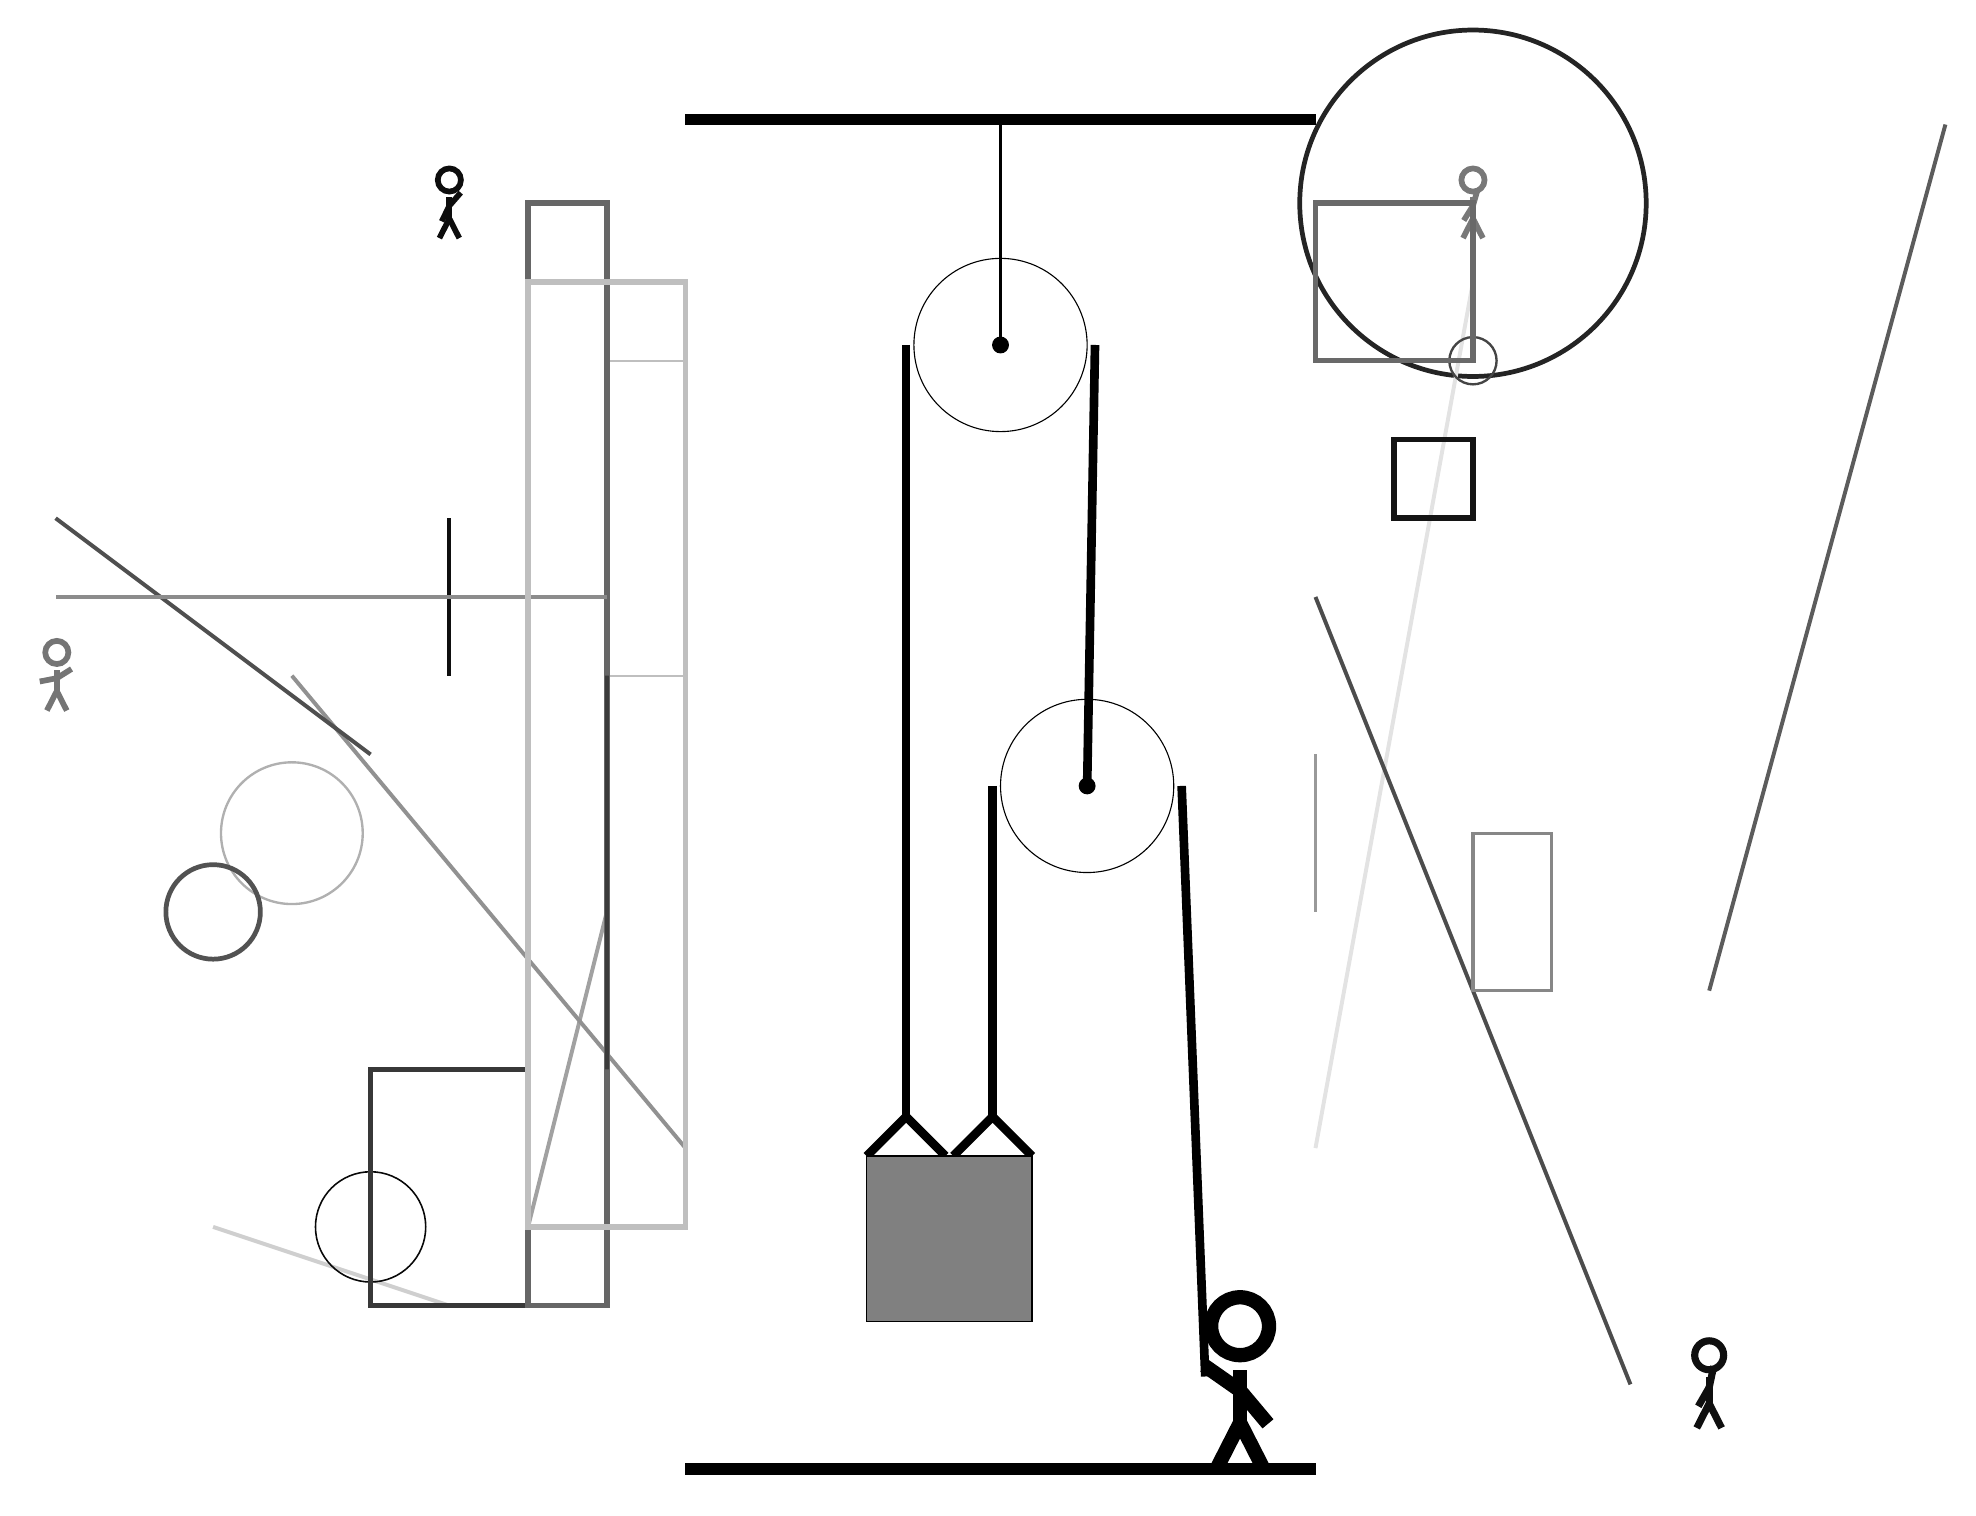
\begin{tikzpicture}
			%%%%% START %%%%%
			
			\draw[fill=black] (-2, 14) rectangle (6, 14.125);
			
			\draw [line width=0.6mm, color=black!86](8, 13) circle (2.2);
			
			\draw [line width=0.3mm, color=black!31](-7, 5) circle (0.9);
			\draw[line width=0.3mm, color=black!25] (-3, 7) rectangle (-2, 11);
			\draw[line width=0.5mm, color=black!64](11, 3) -- (14, 14);
			\draw[line width=0.5mm, color=black!11](8, 12) -- (6, 1);
			
			\draw[line width=0.5mm, color=black!37](-4, 0) -- (-3, 4);
			\draw [line width=0.3mm, color=black!73](8, 11) circle (0.3);
			\draw[line width=0.5mm, color=black!40](6, 4) -- (6, 6);
			\node[line width=0.5mm, color=black!53] at (8, 13) {\Strichmaxerl[4][58][74]};
			\node[line width=0.4mm, color=black!94] at (11, -2) {\Strichmaxerl[5][60][78]};
			
			\draw[line width=0.5mm, color=black!43](-7, 7) -- (-2, 1);
			
			\draw[line width=0.5mm, color=black!19](-5, -1) -- (-8, 0);
			\draw[line width=0.5mm, color=black!94](-5, 7) -- (-5, 9);
			\draw[line width=0.5mm, color=black!70](10, -2) -- (6, 8);
			\draw [line width=0.2mm, color=black!97](-6, 0) circle (0.7);
			\draw[line width=0.6mm, color=black!78] (-4, -1) rectangle (-6, 2);
			\draw[line width=0.7mm, color=black!59] (6, 13) rectangle (8, 11);
			
			\draw [line width=0.6mm, color=black!68](-8, 4) circle (0.6);
			\draw[line width=0.7mm, color=black!60] (-4, 13) rectangle (-3, -1);
			
			\draw[line width=0.4mm, color=black!47] (8, 5) rectangle (9, 3);
			\draw[line width=0.7mm, color=black!92] (7, 10) rectangle (8, 9);
			\draw [line width=0.6mm, color=black!10](9, 9) circle (0.0);
			\draw[line width=0.5mm, color=black!69](-6, 6) -- (-10, 9);
			\draw[line width=0.5mm, color=black!45](-3, 8) -- (-10, 8);
			\draw[line width=0.5mm, color=black!77] (-3, 7) rectangle (-3, 2);
			
			\draw[line width=0.7mm, color=black!25] (-4, 12) rectangle (-2, 0);
			\node[line width=0.6mm, color=black!95] at (-5, 13) {\Strichmaxerl[4][64][49]};
			\node[line width=0.3mm, color=black!54] at (-10, 7) {\Strichmaxerl[4][11][32]};
			
			\draw (2, 11.2) circle (1.1);
			\draw[fill=black] (2, 11.2) circle (0.1);
			\draw[thick] (2, 11.2) -- (2, 14);
			
			\draw (3.1, 5.6) circle (1.1);
			\draw[fill=black] (3.1, 5.6) circle (0.1);
			
			\draw[line width = 1.1mm]  (0.3, 0.9) -- (0.8, 1.4) -- (1.3, 0.9);
			\draw[line width = 1.1mm]  (1.4, 0.9) -- (1.9, 1.4) -- (2.4, 0.9);
			\draw[fill=black!50] (0.3, 0.9) rectangle (2.4, -1.2);
			
			\draw[line width = 1.1mm] (0.8, 11.2) -- (0.8, 1.4);
			\centerarc[line width = 1.1mm](2, 11.2)(0:180:1.2000000000000002);
			\draw[line width = 1.1mm] (3.2, 11.2) -- (3.1, 5.6);
			\draw[line width = 1.1mm] (1.9, 5.6) -- (1.9, 1.4);
			\centerarc[line width = 1.1mm](3.1, 5.6)(0:180:1.2000000000000002);
			\draw[line width = 1.1mm] (4.3, 5.6) -- (4.6, -1.9);
			
			\node at (5, -2) {\Strichmaxerl[10][-35][-50]};
			
			\draw[fill=black] (-2, -3) rectangle (6, -3.15);
			
			%%%%% END %%%%%
		\end{tikzpicture}
	\end{figure}	
\end{document}